% Draft of the final report, Project in Data Science (1DL507), HT2026.
% First draft: 10 November 2026. Decisions of 12 November 2026 recorded; every number is from before
% the corrections and is replaced after the rerun (finishing plan B4, B6).
% Every \todo marks something the group still has to decide,
% check or fill in. Numbers come from the result files named in report/README.md.
%
% The course asks for its own LaTeX conference template (Canvas, Templates page). This file
% uses the standard IEEE conference class as a stand-in; move the body into the course
% template before submission.
\documentclass[conference]{IEEEtran}

\usepackage[utf8]{inputenc}
\usepackage[T1]{fontenc}
\usepackage{amsmath}
\usepackage{booktabs}
\usepackage{graphicx}
\usepackage{xcolor}
\usepackage{url}
\usepackage{siunitx}
\sisetup{detect-all}

\newcommand{\todo}[1]{\textcolor{red}{[TODO: #1]}}
\newcommand{\cdelay}{\texttt{current\_delay}}

\begin{document}

\title{How Early Can a Disrupted Train Journey Be Foreseen?\\
Severity and Delay Prediction for Frankfurt--M\"unchen\\ With and Without Weather}

\author{\IEEEauthorblockN{\todo{Name 1}, \todo{Name 2} and \todo{Name 3}\thanks{Division of work:
\todo{one sentence per author, for text and for code; the course requires this, see
ProjectInstructions.md, ``Final report'' and ``Code and scripts''}. Supervisor: Qing He, Mid Sweden
University.}}
\IEEEauthorblockA{Project in Data Science (1DL507), Uppsala University, HT2026}}

\maketitle

\begin{abstract}
A passenger who knows a day ahead that a long-distance train is likely to be badly delayed or
cancelled can take an earlier train or another route. We study how well this can be predicted for
direct ICE and IC journeys from Frankfurt (Main) Hbf to M\"unchen Hbf, using 21{,}831 journeys from
July 2024 to September 2026. At five times between 24 hours and 0 minutes before the scheduled
departure we predict the arrival delay in minutes and the probability of four severity classes
(under 20 minutes, 20 to 59 minutes, 60 minutes or more, cancelled). Every input is restricted to
what an archive of live updates shows was known at the prediction time. Under this restriction,
gradient-boosted trees lower the multi-class log loss from 0.968 (class shares) to 0.920 at
24 hours and from 0.897 to 0.819 at departure, and the delay error by 4 to 7\%. The reliability of
the same service over the previous weeks is the most useful new input. Hourly weather observations
along the route do not improve either prediction: on 23 held-out weeks, all ten paired 95\%
intervals for the change include zero.
\end{abstract}

\section{Introduction}

Long-distance trains in Germany are often late. On the route studied here, one journey in four
arrives 20 to 59 minutes late, and more than one in ten arrives at least an hour late or does not
run as planned. For a passenger, the average delay matters less than the risk of a serious disruption: a
missed connection, an appointment or a flight. A useful forecast is therefore a probability of
disruption, given early enough that the passenger can still change plans.

This project asks how likely a journey is to suffer a serious disruption, and how that estimate
changes as the departure approaches. We consider direct ICE and IC journeys between one selected
origin--destination pair, Frankfurt (Main) Hbf to M\"unchen Hbf, and answer three questions:

\begin{enumerate}
\item How accurately can the arrival delay and the disruption severity of a journey be predicted
24~h, 6~h, 1~h, 20~min and 0~min before its scheduled departure?
\item Does weather along the route improve these predictions over railway information alone?
\item Which information carries the prediction at each of these times, and how does the predicted
risk of a journey change between them?
\end{enumerate}

We build a journey dataset from public records of Deutsche Bahn train movements and from station
observations of the German weather service (DWD). Standard models (logistic and linear regression,
random forests, gradient-boosted trees) and a range of further model families are compared under one
evaluation protocol. The comparison of railway-only models with railway-plus-weather models uses the
same journeys, the same models and the same search budget, and is confirmed once on held-out weeks.

Three results stand out. First, the predictions beat simple references at every prediction time, but
by a modest margin, and journeys that end 60 minutes or more late are predicted poorly. Second,
weather observations add nothing measurable. Third, the definition of ``known at the prediction
time'' changes the apparent accuracy more than any choice of model does.

Section~\ref{sec:related} relates the work to earlier studies. Section~\ref{sec:method} defines the
prediction task, the inputs, the models and the evaluation. Section~\ref{sec:results} describes the
data and reports the results, and Section~\ref{sec:discussion} discusses them and their limitations.

\section{Related Work}
\label{sec:related}

Spanninger et al.~\cite{spanninger2022review} review train delay prediction and classify approaches
by what is predicted (a delay at a later stop, or an event time), by the prediction horizon, and by
whether the output is a single value or a distribution. Most studies predict the delay at one of the
next stops from the current delay, minutes ahead. Li et al.~\cite{li2021nearterm} do so for the
Dutch network about 20 minutes ahead with random forests, gradient boosting and neural networks, and
find the current delay to be by far the most important input. Our setting differs in two ways: the
target is the arrival at the passenger's destination several hours later, and four of our five
prediction times lie before the train has left the passenger's origin.

Fewer studies predict a probability of a class of outcome. Jiang et al.~\cite{jiang2019punctuality}
predict the punctuality at the final stop in Sweden by combining a logistic model with a random
forest, with a threshold of about six minutes. Cancellations are usually removed from the data; we
keep them as a class of their own, because for the passenger they are the worst outcome.

The value of weather has been studied with mixed results. Oneto et
al.~\cite{oneto2016weather} add weather observations and forecasts to a delay prediction system for
the Italian network and report better accuracy. Huang et al.~\cite{huang2020sequences} combine
operational and weather data in a sequence model for Chinese high-speed lines. In contrast,
Spanninger et al.~\cite{spanninger2024predictability} \todo{check the exact statement in the paper
before citing it for ``weather did not help''}. \todo{Add two or three of the weather studies from
literature\_review/regression\_models.md and classification\_models.md once someone has read the
full texts.}

Network-wide models such as the transformer of Arthaud et al.~\cite{arthaud2024transformers} use the
state of all trains at once. We work with one origin--destination pair and tabular models, where
gradient-boosted trees are known to be hard to beat~\cite{grinsztajn2022trees}. For the evaluation
we follow the recommendation of Tiong et al.~\cite{tiong2025apgrip} to look beyond one accuracy
figure: we report performance by prediction time, by outcome class and by period, and we separate
the error on completed journeys from the classification of disruptions.

\section{Methodology}
\label{sec:method}

\subsection{Prediction task}

A \emph{journey} is one dated run of one ICE or IC train that stops at Frankfurt (Main) Hbf and
later at M\"unchen Hbf. For each journey we predict two targets. The \emph{arrival delay} is the
reported minus the planned arrival time at M\"unchen Hbf in minutes; it is defined for completed
journeys only. The \emph{severity class} is one of: under 20~min, 20 to 59~min, 60~min or more, and
cancelled. A journey counts as cancelled when its departure from Frankfurt or its arrival in
M\"unchen is cancelled; a cancellation at an intermediate stop alone does not count.

Predictions are made at five \emph{prediction times}: 24~h, 6~h, 1~h, 20~min and 0~min before the
scheduled departure from Frankfurt. No prediction is made for a journey whose cancellation has
already been announced at that time, since the passenger then knows the outcome. A separate model is
fitted for each prediction time and each target.

\subsection{Inputs known at the prediction time}
\label{sec:inputs}

The monthly files of the source keep, for every stop, only the last reported values. They do not say
when a value became known. A model trained on them can therefore use information from after the
prediction time without anyone noticing. Two examples: the stops recorded for a journey (their
number and the route they form) depend on the outcome, because a diverted or curtailed train records
different stops; and the delay of the train on its way to Frankfurt, as it stands in the final
records, need not have been reported by the prediction time.

All results in this report therefore use inputs reconstructed from the
archive of live-update snapshots of the same source. An event counts as known only if a snapshot
requested at or before the prediction time shows it. The inputs fall into the following groups.

\begin{itemize}
\item \emph{Timetable and calendar:} planned travel time, planned number of stops, planned minutes
the run has travelled before Frankfurt, train type, whether the run starts in Frankfurt, a planned
route identifier, and the hour, weekday and month of the departure.
\item \emph{Holidays:} public and school holidays in Hesse, Baden-W\"urttemberg and Bavaria, bridge
days, and the days before and after a holiday.
\item \emph{Recent reliability:} for the same scheduled service, the share of severe or cancelled
journeys and the mean delay over the last 7 and 28 days; for all journeys of the pair, the same over
the last 3 and 24 hours.
\item \emph{Current delay} (from 1~h on): the latest delay of the run reported by the prediction
time, its change since the previous prediction time, the number of stops reported, and the planned
minutes still to run before Frankfurt.
\item \emph{Network state:} the share of long-distance trains delayed by 20~min or more or cancelled
in the previous hour, over the network, at Frankfurt Hbf and at M\"unchen Hbf.
\item \emph{Weather:} 14 values from hourly DWD observations at the stations along the route, for
the last full hour before the prediction time: temperature at both ends, the highest and lowest
temperature, the highest precipitation, mean wind and gust on the route in that hour and over the
previous 24 hours, snow depth, and whether snow fell.
\end{itemize}

The route used for the weather is a fixed list of stations for each of the two branches (via
N\"urnberg and via Stuttgart), chosen by the timetable of the scheduled train, not by the stops the
journey recorded. The weather is observed weather; a forecast for the time of travel is not used
(Section~\ref{sec:limits}).

\subsection{Models}

Two references need no features: the class shares of the training journeys, and their mean delay.
The standard models are multinomial logistic regression and linear regression, a random forest
\cite{breiman2001forests}, XGBoost~\cite{chen2016xgboost}, LightGBM~\cite{ke2017lightgbm} and, for
the delay only, support vector regression. Linear models receive standardised numeric inputs,
one-hot encoded categories, and a missing \cdelay{} as zero with an indicator. Tree models receive
missing values as such; the two boosting libraries split on categories directly.

Beyond these we tested, as planned extensions: CatBoost~\cite{prokhorenkova2018catboost}; an
explainable boosting machine~\cite{nori2019interpretml}; two-stage models that first predict
cancellation and then the delay class or the delay distribution; ensembles (averages, greedy
weighting, stacking); probability calibration; multilayer perceptrons, including a multi-task
network for both targets, an architecture search with gated neurons~\cite{orucu2026tabgns},
RealMLP~\cite{holzmuller2024realmlp} and TabM~\cite{gorishniy2025tabm}; a recurrent network over the
stops before Frankfurt; one model pooled over all prediction times; and transfer from three other
origin--destination pairs and from all long-distance runs in the network. The work was implemented
in Python with scikit-learn~\cite{pedregosa2011sklearn}, LightGBM, XGBoost and PyTorch.

\subsection{Evaluation}
\label{sec:evaluation}

\emph{Split.} With about two years of data, a chronological split would test on a single season. We
instead split by ISO week: all journeys of a week are on the same side, because weather, strikes and
construction work affect neighbouring days together. Of 118 weeks, 23 form a hold-out set and 95 a
cross-validation (CV) set, divided into five folds of whole weeks. Weeks were assigned by a
stratified group split on the severity class, and the assignment was fixed before any model was
fitted. \todo{State that this split was agreed with the supervisor on 12 October 2026, or leave it
out.}

\emph{Metrics.} Severity models are chosen by the multi-class log loss, which judges the predicted
probabilities; we also report macro-F1 of the most probable class. Delay models are scored by the
root mean squared error (RMSE) in minutes on completed journeys.

\emph{Tuning.} Hyperparameters were chosen by random search (20 configurations for the boosted
trees, eight for the neural networks). For results reported as findings the search is nested: each
of the five outer folds chooses its configuration, and where applicable its feature groups, on four
inner folds of its own training weeks. Results with a configuration reused from an earlier search
are labelled exploratory.

\emph{Comparing models.} The five folds share training weeks, so their score differences are not
independent and a paired $t$-test on them is too
optimistic~\cite{bengio2004variance}. We report the mean of the five paired differences and the
number of folds that improve. Before screening, we fixed the smallest difference that we count as a
gain: 0.003 in log loss and 0.1~min in RMSE, two to three times the measured optimism of a
non-nested search.

\emph{Hold-out evaluation.} Before the hold-out set was opened, one pair of models was registered
for each target and prediction time: the pipeline with the best railway-only CV score, and the same
pipeline with the weather inputs added and tuned with the same budget. Each model was refitted on
the 95 CV weeks and scored once on the 23 hold-out weeks. Intervals for the difference between the
two arms come from 2{,}000 paired bootstrap resamples of whole weeks.

\section{Results}
\label{sec:results}

\subsection{Dataset}

Railway data come from a public archive of Deutsche Bahn timetable and live-update
records~\cite{piebro_db_data}, of which monthly files exist from July 2024. The
Bahn-Vorhersage data named in the project description had not been made available to us by its
owners. We use the
27 months to September 2026. After keeping one journey per departure (a cancelled train and its
replacement at the same times are one departure for the passenger) and dropping 193 unusual journeys
(a detour of about nine hours via K\"oln, and trains for which Frankfurt or M\"unchen was an added
stop), 21{,}831 journeys remain: 17{,}507 in the CV set and 4{,}324 in the hold-out set. Weather
comes from hourly observations of the DWD Climate Data Center~\cite{dwd_cdc} at stations near the
15 railway stations on the two branches, with gaps filled from a second station within 50~km.

In the CV set, 62.8\% of journeys arrive less than 20~min late, 25.5\% arrive 20 to 59~min late,
6.2\% arrive 60~min or more late, and 5.5\% are cancelled. Completed journeys are on average
18.4~min late (median 10~min, 95th percentile 67~min, maximum 279~min). Table~\ref{tab:data} shows
how the cohort changes with the prediction time. Of the 956 cancellations in the CV set, 41\% had
been announced one hour before departure and 59\% by the scheduled departure, so the share of
cancellations still to be predicted falls from 5.2\% to 2.3\%.

The table also shows the effect of the restriction of Section~\ref{sec:inputs}. One hour before
departure the final records contain a delay of the run for 86\% of the journeys, but the archive
shows a report requested by that time for only 39\%. The gap comes from how often the archive was
fetched: live updates were requested in blocks about six hours apart, so for most journeys the last
request before the prediction time came before the train had reported from any stop on its way to
Frankfurt. In a sample of the journeys without an archive value, the first report of the run arrived
a median of 1.9~h after the prediction time. Where both versions have a value, the archive version is
lower in 58\% of the rows and equal in about a third, and the difference grows with the age of the
latest report, from a mean of $-1.0$~min when it is under 30 minutes old to $-11.7$~min when it is
over four hours old. The final records thus overstate what was known: they treat every report as
visible the moment the event happened. \todo{Q5: the group decides whether the report gives the
archive version only or both versions of the current delay.}

\begin{table}[t]
\caption{Prediction rows in the CV set by prediction time, and the share for which a delay of the
run before Frankfurt is available}
\label{tab:data}
\centering
\footnotesize
\setlength{\tabcolsep}{3.5pt}
\begin{tabular}{@{}lrrrrr@{}}
\toprule
 & 24 h & 6 h & 1 h & 20 min & 0 min \\
\midrule
Journeys predicted & 17{,}463 & 17{,}366 & 17{,}096 & 16{,}975 & 16{,}926 \\
Of these cancelled (\%) & 5.2 & 4.8 & 3.3 & 2.6 & 2.3 \\
Delay in final records (\%) & 0 & 5 & 86 & 87 & 87 \\
Delay in archive (\%) & -- & -- & 39 & 43 & 52 \\
\bottomrule
\end{tabular}
\end{table}

\subsection{Experimental setup}

All experiments ran on one laptop (\todo{model, processor, memory}; Python~3.13, scikit-learn~1.9,
LightGBM~4.7, XGBoost~3.4, PyTorch~2.9). Models were fitted single-threaded with fixed seeds.
The cross-validation experiments comprise 366 model arms. \todo{Total computing time, if we can
reconstruct it from the run logs.}

\subsection{Predictability by prediction time}

Fig.~\ref{fig:scores} and Table~\ref{tab:cv} show the CV scores. All models beat the references at
every prediction time. A day ahead, LightGBM with the feature groups chosen inside each fold
lowers the log loss from 0.968 to 0.920 and the RMSE from 25.4 to 24.4~min. At departure it reaches
0.819 and 23.6~min. Most of the fall in log loss is not better prediction: the reference itself
falls from 0.968 to 0.897, because announced cancellations leave the cohort. Against the reference,
the gain grows from 0.048 at 24~h (5\%) to 0.078 at departure (9\%). The delay scores use the same
completed journeys at every prediction time, so their trend is not affected.

In absolute terms the predictions remain weak. Macro-F1 stays below 0.29 at every prediction time,
since ``under 20~min'' is the most probable class for almost every journey. The delay models explain
little of the variation: an RMSE of 23.6~min compares with a standard deviation of 25.4~min.

\begin{figure*}[t]
\centering
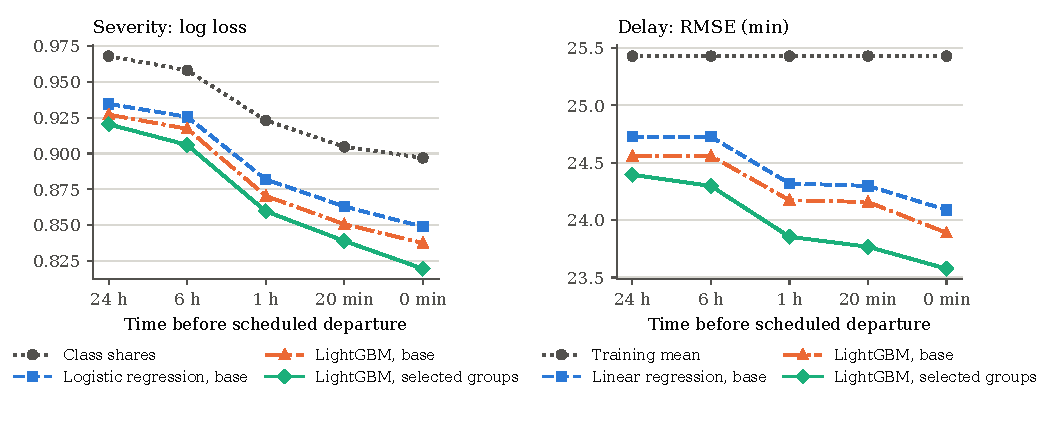
\includegraphics[width=0.92\textwidth]{figures/fig_scores.pdf}
\caption{Cross-validation scores at the five prediction times (mean of five week folds; lower is
better). ``Base'' uses timetable and calendar inputs, with the current delay from 1~h on. ``Selected
groups'' adds the feature groups of Section~\ref{sec:inputs} without weather, chosen inside each
outer fold.}
\label{fig:scores}
\end{figure*}

\begin{table}[t]
\caption{Scores by prediction time. CV: mean of five folds, nested tuning for LightGBM.
Hold-out: registered railway-only models}
\label{tab:cv}
\centering
\footnotesize
\setlength{\tabcolsep}{3.5pt}
\begin{tabular}{@{}lrrrrr@{}}
\toprule
 & 24 h & 6 h & 1 h & 20 min & 0 min \\
\midrule
\multicolumn{6}{@{}l}{\emph{Severity, log loss}} \\
Class shares (CV) & 0.968 & 0.958 & 0.923 & 0.905 & 0.897 \\
Logistic regr., base (CV) & 0.935 & 0.926 & 0.882 & 0.863 & 0.849 \\
LightGBM, base (CV) & 0.927 & 0.917 & 0.870 & 0.851 & 0.837 \\
LightGBM, sel. groups (CV) & 0.920 & 0.906 & 0.860 & 0.839 & 0.819 \\
Registered model (hold-out) & 0.920 & 0.907 & 0.863 & 0.840 & 0.820 \\
\midrule
\multicolumn{6}{@{}l}{\emph{Delay, RMSE (min)}} \\
Training mean (CV) & 25.43 & 25.43 & 25.43 & 25.43 & 25.43 \\
Linear regr., base (CV) & 24.73 & 24.73 & 24.32 & 24.30 & 24.09 \\
LightGBM, base (CV) & 24.56 & 24.56 & 24.17 & 24.16 & 23.89 \\
LightGBM, sel. groups (CV) & 24.39 & 24.30 & 23.85 & 23.77 & 23.58 \\
Registered model (hold-out) & 25.15 & 25.03 & 24.61 & 24.49 & 24.27 \\
\bottomrule
\end{tabular}
\end{table}

On the hold-out weeks the severity scores of the registered models agree with the CV scores
recorded at registration to within 0.003. The delay errors are 0.7~min higher than those CV scores
at every prediction time. \todo{All numbers in this section are from before the corrections decided on 12 November.
Replace the tables, the figures and this paragraph after the rerun and the second hold-out
evaluation (finishing plan B4, B6), and add the two reference scores on the hold-out set (class
shares and training mean).}

\subsection{Which inputs help}

Added one group at a time to the base inputs, recent reliability is the only group that reaches the
minimum gain consistently: in 17 of 20 comparisons (two models, two targets, five prediction times),
by 0.010 to 0.018 in log loss and 0.30 to 0.45~min in RMSE for the linear models. Holidays and
network state never reach it, the planned-timetable inputs once and the delay dynamics twice. In the
nested comparison, letting each outer fold choose its feature groups improves LightGBM over the base
inputs at all five prediction times for both targets (Table~\ref{tab:cv}). Because the reliability
inputs were screened on the same five folds before the nested comparison was specified, the size of
the gain is more certain than its exact ranking among the groups.

Permutation importance by group shows how the useful information shifts: calendar inputs lead at
24~h, recent reliability at 6~h, and the current delay close to departure. \todo{One sentence on the
SHAP ranking (departure hour first) and what it means.}

\subsection{Model families}

Gradient-boosted trees are slightly better than the linear models, by 0.008 to 0.012 in log loss
and 0.14 to 0.20~min in RMSE on the base inputs. None of the further model families improved on
LightGBM by the minimum gain: CatBoost, the explainable boosting machine, the two-stage and ordinal
models, the mixture of experts, the distributional models, calibration, weighted ensembles and
stacking never reached it. None of the neural networks improved on LightGBM in any of 112
comparisons on the same inputs; the closest came within 0.009 in log loss and 0.03~min. Averaging
over seeds and configurations reached the minimum gain in 8 of 120 comparisons. Pooling the
prediction times reached it in 6 of 20, all in the weather arm and none against the railway-only
model per prediction time. With this many comparisons on the same five folds we do not read these
as gains. For the delay
at 6~h, 1~h and 20~min a linear regression on all feature groups had the best railway-only CV score
and was registered as the final model. \todo{Decide how much of the neural-network comparison to
report. RealMLP, TabM and the gated architecture search improved on the plain MLP in part of the
comparisons, but not on LightGBM. Three arms did not fit properly (the mixture model of the
distributional family, the explainable boosting machine with weather for delay at 24~h, the TabM
classifier at 24~h) and should be described as failed, not as ``no gain''.}

\subsection{Does weather help?}

We found no improvement. Table~\ref{tab:weather} and Fig.~\ref{fig:weather} give the hold-out
result for the ten registered pairs. Adding the weather inputs changes the log loss by between $-0.001$ and $+0.005$
and raises the RMSE by 0.02 to 0.19~min. All ten 95\% intervals include zero, and eight of the ten
point estimates go against weather. The same holds in cross-validation for every model we tried:
logistic and linear regression, random forest, XGBoost, LightGBM and support vector regression
gained nothing from the weather inputs, and no pre-specified subset of them (temperature only, wind
only, snow only, indicators of extremes) changed this.

\begin{table}[t]
\caption{Hold-out set: railway plus weather minus railway only, with 95\% intervals from a
paired bootstrap of 23 weeks. Negative values favour weather}
\label{tab:weather}
\centering
\footnotesize
\setlength{\tabcolsep}{3.5pt}
\begin{tabular}{@{}lrlrl@{}}
\toprule
 & \multicolumn{2}{c}{Severity, log loss} & \multicolumn{2}{c}{Delay, RMSE (min)} \\
\cmidrule(lr){2-3}\cmidrule(l){4-5}
 & $\Delta$ & 95\% interval & $\Delta$ & 95\% interval \\
\midrule
24 h & $+0.0049$ & $[-0.0014, +0.0112]$ & $+0.19$ & $[-0.01, +0.40]$ \\
6 h & $-0.0009$ & $[-0.0062, +0.0038]$ & $+0.08$ & $[-0.03, +0.17]$ \\
1 h & $+0.0006$ & $[-0.0028, +0.0039]$ & $+0.08$ & $[-0.02, +0.18]$ \\
20 min & $+0.0011$ & $[-0.0028, +0.0049]$ & $+0.11$ & $[-0.01, +0.24]$ \\
0 min & $-0.0000$ & $[-0.0032, +0.0035]$ & $+0.02$ & $[-0.13, +0.17]$ \\
\bottomrule
\end{tabular}
\end{table}

\begin{figure}[t]
\centering
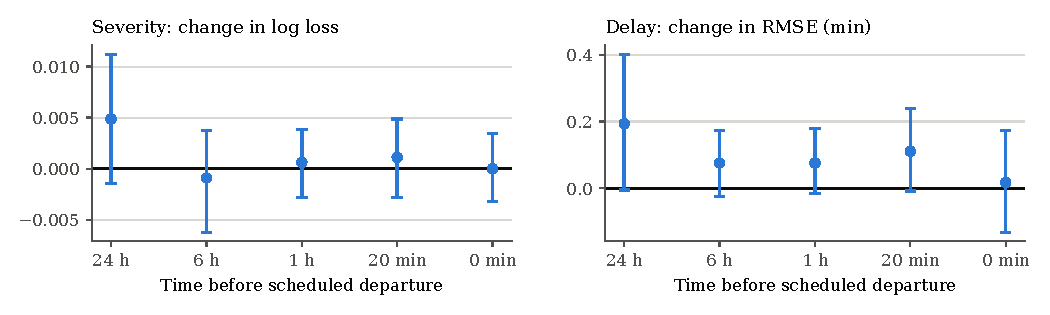
\includegraphics[width=\columnwidth]{figures/fig_weather.pdf}
\caption{Hold-out change in score when weather inputs are added (points) with paired 95\% bootstrap
intervals over weeks. Values above zero mean that weather made the prediction worse.}
\label{fig:weather}
\end{figure}

Three properties of this comparison limit what it shows. With 23 weeks, the intervals exclude gains
larger than about 0.003 to 0.006 in log loss and 0.13~min in RMSE, not smaller ones; they are
pointwise for ten related comparisons. The route aggregates were available for
57 to 65\% of the rows. For most journeys from November 2025 on, the archive holds no timetable
record requested before the prediction time, so the branch of the journey is unknown and only the
temperatures at the two ends were used. \todo{From the rerun on, the timetable of these journeys is treated as static, as for the
earlier period (decision of 12 November); rewrite these two sentences with the new coverage.} And days with extreme weather are rare: the groups with heavy rain contain two to four
hold-out journeys per prediction time, so nothing can be said about them.

\subsection{Errors and risk over time}

The errors are concentrated in the rare classes. On the hold-out set, the delay model at 24~h has an
RMSE of 14.9~min on journeys that arrive less than 20~min late and 74.1~min on those that arrive
60~min or more late: severe delays are predicted far too low at every prediction time. For severe
delays and cancellations, predicted probabilities above 0.5 hardly occur, so the calibration of the
upper range cannot be judged. \todo{Add the share of squared error caused by the 60+~min journeys
for the final models.}

The predicted risk of a single journey moves little before departure. For example, for one journey
that ended more than an hour late, the predicted probability of ``60~min or more or cancelled'' was
10\% at 24~h, 18\% at 6~h and 10\% at departure. \todo{Replace the single example with a summary
over all hold-out journeys: how much the predicted probability of a severe disruption changes
between 24~h and 0~min, for journeys that were and were not severely disrupted.}

\section{Discussion}
\label{sec:discussion}

\subsection{Findings}

\emph{Disruptions are only weakly predictable before departure.} A day ahead, the time of day, the
weekday and the recent record of the service separate more and less reliable journeys, and this is
worth about 5\% of the log loss. Closer to departure the delay of the incoming train helps where it
is known. But the events that matter most to a passenger, a delay of an hour or a cancellation, are
mostly caused by incidents that have not yet happened or are not visible in our inputs, and the
models fall back on the average.

\emph{Weather observations do not help.} This is in line with \todo{cite after checking} and
differs from Oneto et al.~\cite{oneto2016weather}. Several explanations are possible, and our data
cannot separate them. Weather that disrupts trains is rare and local, so two years on one route
contain few examples. The recent reliability of the service and the state of the network already
reflect a disruption once it has begun, whatever its cause. And we used the weather at the time of
the prediction, which a day ahead says little about the weather during the journey.

\emph{Information matters more than the learner.} Adding the recent reliability of a service
improved a linear model more than replacing it by any other model family did. On about ten to thirty
tabular inputs, tuned boosted trees, neural networks and ensembles ended within noise of each other.

\subsection{Limitations}
\label{sec:limits}

\emph{Scope.} The results hold for one origin--destination pair in one direction and for 27 months.
All prediction times lie at or before the departure; updates during the journey were not studied.

\emph{Split.} The split by week is not chronological. Models are trained on weeks after the weeks
they are tested on, so the scores describe interpolation within the period, not a forecast for the
following year. Recent-reliability inputs may use earlier journeys from hold-out weeks, as a
deployed system would.

\emph{Known at the prediction time.} The archive bounds what we can show was known, not what Deutsche
Bahn's own systems knew. Timetable fields are treated as static, whatever their request time in the archive. DWD observations were assumed to be available at the end of their hour.

\emph{Weather.} Observations were used, not forecasts. A forecast for the hours of the journey might
carry information that the weather at the prediction time does not.

\emph{Labels.} A small number of arrival times are forecasts made shortly before arrival, mostly in
summer 2026 (132 of 21{,}800 checked journeys), and from October 2025 the source reports arrivals of
exactly 0~min more often than before.

\subsection{Societal and ethical aspects}

\todo{The syllabus asks for this. Points to consider: a risk estimate that is weak but presented
with confidence can mislead passengers; advice to avoid certain trains shifts demand and may crowd
others; the data are public operational records without personal data; the use of an AI coding
assistant in this project and how its output was checked.}

\subsection{Future work}

The most direct extensions are weather forecasts for the time of travel in place of observations;
prediction times after departure, where the brief asks how risk updates during the journey; and more
origin--destination pairs with a longer history, which would permit a chronological test. Since the
severe class drives both the error and the value to passengers, causes of disruption that are known
in advance, such as planned construction work and strikes, are the most promising missing input.

\section{Conclusion}

For direct long-distance journeys from Frankfurt to M\"unchen, the severity of a disruption and the
arrival delay can be predicted better than by historical averages from 24 hours before departure,
but only modestly: the log loss improves by 5\% a day ahead and by 9\% at departure. The recent
reliability of the service is the most useful input beyond the timetable, gradient-boosted trees and
linear models are close, and nothing more elaborate did better. Weather observations along the route
gave no detectable improvement in cross-validation or on held-out weeks.

\bibliographystyle{IEEEtran}
\bibliography{references}

\end{document}
